%% Page settings.
\documentclass[10pt,a4paper,twoside]{article}
\usepackage[top=1.2in, left=1.2in, bottom=1.2in, right=1.2in]{geometry}
%==================================================%
%% Encoding packages.
\usepackage[UKenglish]{babel}
\usepackage[nodayofweek]{datetime}
\usepackage[T1]{fontenc}
\usepackage[utf8]{inputenc}
\usepackage{amsmath}
\usepackage{amsthm}
\DeclareMathAlphabet\mathbb{U}{msb}{m}{n}
%\usepackage{amsfonts}
\usepackage{amssymb}
\usepackage{calc}
\usepackage{natbib}
\usepackage{color}
\usepackage{subcaption}
%==================================================%
%% Document details.
\usepackage{titling}
\title{Information and admissible sets}
\author{Jeff Rowley}
\newcommand{\thedate}{\today}
% Enter document details here.
\newcommand{\details}{C:/Users/Jeffro/Dropbox/TeXTemplates/}
% Enter the file path here for the UCL logo and bibliography.
% Change this file path for different computer systems.
\newcommand{\homePC}{C:/Users/Jeffro/Documents/}
\newcommand{\workPC}{U:/}
%==================================================%
%% Date macro.
\newcommand{\theseason}[1]{
\ifcase \month 
\or Winter\or Winter\or Spring\or Spring\or Spring\or Summer\or Summer\or Summer\or Autumn\or Autumn\or Autumn\or Winter\fi}
% Displays the season.
% Obsolete in this template.
%==================================================%
%% Useful packages.
\usepackage{enumerate}		% Lists.
\usepackage{bbm}			% Indicator functions.
\usepackage{lipsum}			% Random text generator.
\usepackage{MnSymbol}		% Arrows.
\usepackage{graphicx}		% Graphics.
\usepackage{mathtools}		% Math*lap command.
 \usepackage{booktabs}
 \usepackage{multirow}
 \usepackage{rotating}
%==================================================%
%% Theorem environments.
\newcounter{countthm}[section]
\newcounter{countlem}[section]
\newcounter{countex}[section]
% Creates new counters which reset at each new section. 
\renewcommand{\thecountthm}{\thesection.\arabic{countthm}}
\renewcommand{\thecountlem}{\thesection.\arabic{countlem}}
\renewcommand{\thecountex}{\thesection.\arabic{countex}}
% Redefines counters to include the section number.
\newtheorem{thm}[countthm]{Theorem}
% Creates a theorem environment - type \thm to begin.
\newtheorem{lem}[countlem]{Lemma}
% Creates a lemma environment - type \lem to begin.
\newtheorem{ex}[countex]{Example}
% Creates an example environment - type \ex to begin.
\newtheorem*{Acknowledgements}{Acknowledgements}
% Creates a thanks environment.
\newcommand{\newthm}[1]{\newtheorem*{#1}{#1}}
% A macro that makes defining new theorem environments quick.
% Type \newthm{<Theorem name here>} to begin.
%==================================================%
%% Math operators.
\DeclareMathOperator*{\plim}{plim}
% Writes plim in math environment - type \plim to enter.
\DeclareMathOperator*{\argmax}{argmax}
% Writes argmax in math environment - type \argmax to enter.
\DeclareMathOperator*{\argmin}{argmin}
% Writes argmin in math environment - type \argmin to enter.
\DeclareMathOperator*{\argsup}{argsup}
% Writes argsup in math environment - type \argsup to enter.
\DeclareMathOperator*{\arginf}{arginf}
% Writes arginf in math environment - type \arginf to enter.
\newcommand\independent{\protect\mathpalette{\protect\independenT}{\perp}} 
\def\independenT#1#2{\mathrel{\rlap{$#1#2$}\mkern2mu{#1#2}}} 
% Pastes an independence symbol - type \independent to enter.
\DeclareMathOperator*{\generates}{:.}
% Write generate symbol (identification).
\DeclareMathOperator*{\generated}{.:}
% Write generated symbol (identification).
%==================================================%
%% Abbreviations.
\newcommand{\US}{United States}
% Use \US macro when use is as a noun.
% Use U.S. when use is as an adjective.
%==================================================%
%% Equation numbering.
\numberwithin{equation}{section}
% Numbers equations up to the subsection. To change level,
% replace subsection with section.
%==================================================%
%% Counters.
\newcounter{saveenumi}
\newcounter{saveenumi1}
\setcounter{section}{0}
\newcommand\invisiblesection[1]{%
  \refstepcounter{section}%
  \addcontentsline{toc}{section}{\protect\numberline{\thesection}#1}%
  \sectionmark{#1}}
%==================================================%
\newcommand{\ESRC}{I gratefully acknowledge financial support from the Economic and Social Research Council (ESRC).}
\newcommand{\RLaTeX}{I acknowledge the \emph{R} and \emph{\LaTeX} communities, and the wealth of knowledge that they have made freely available to all.}
%==================================================%
%% The title page.
\makeatletter				
% Changes @ to catcode 11.
\renewcommand{\@maketitle}{
\null
\graphicspath{ {\details} }
\flushleft{\includegraphics[width=40mm]{UCL_Logo_Orange}}
\hspace{5mm}
\normalsize Department of Economics, University College London\\
\vskip\bigskipamount
\leaders\vrule width \textwidth\vskip0.4pt 
\vskip\bigskipamount 
\nointerlineskip
% This completes the UCL banner.
\begin{center}
\begin{minipage}{100mm}
\begin{center}
\vspace{20mm}
\LARGE
\textbf{
\@title}
\par
\vspace{10mm}
\normalsize
\@author
\par
\vspace{5mm}
\normalsize
\thedate
\end{center}
\end{minipage}
\end{center}
}
\makeatother				
% Reverts @ to catcode 12.
%==================================================%
%% Packages to load at end of preamble. 
% Note conflict between Tkz-euclide package set and 
% game theory package set. Load one or the other.
\usepackage{hyperref}
%\usepackage[numbered]{mcode}

%% Tkz-euclide package set.
%\usepackage{tkz-euclide}
%\usepackage{pgfplots}
%\usepgfplotslibrary{external} 
%\tikzexternalize[prefix=tikz/]

%% Game theory package set.
\usepackage{pstricks}	
\usepackage{egameps}		 
\usepackage{pst-3d}			
\usepackage{sgame}	
\renewcommand{\gamestretch}{1.5}
%==================================================%
%% Further notes regarding egameps package.
% The egameps package is incompatible with this template
% due to UCL logo. Solution is to independently run 
% egameps through on a latex blank document, then insert 
% pdf into this document. Recall that to run egameps:
% "latex" --> "DVi->PS" --> "PS->PDF"
% then use "includegraphics[]" with trim option. 
%==================================================%
%% Headers and footers.
\usepackage{fancyhdr}
\pagestyle{fancy}
\renewcommand{\sectionmark}[1]{\markright{\thesection.\ #1}}
% This redefines the \rightmark command so that the section number does not appear.
% NOTE: To remove the section number, delete <<\thesection.\>>
\lhead[\thepage]{\rightmark}
\rhead[\rightmark]{\thepage}
\chead[]{}
\cfoot[]{}
%\lfoot[\thetitle]{}
%\rfoot[]{\theauthor}
\renewcommand*\thesection{\arabic{section}}
\usepackage{epigraph}
%==================================================%
%% Start of document.
\begin{document}
\maketitle
\vspace{10mm}
\begin{abstract}
\noindent <<Abstract here>>
\begin{Acknowledgements}
{\RLaTeX} I thank Andrew Chesher and Toru Kitagawa for their supervision and support. I further thank Adam Rosen for helpful discussion. {\ESRC}
\end{Acknowledgements}
\end{abstract}
\vspace{5mm}
%==================================================%
%% Document.
%==================================================%
I explore the effect of incorporating information for a non-parametric binary choice model. The model permits endogenous variation in a scalar random variable that is due to non-random selection, and it is the average causal effect of this endogenous variable on the outcome variable that is of interest. The model embeds an exclusion restriction and an independence restriction that together define an instrumental variable but is silent as to the relationship between the endogenous variable and the instrumental variable. I restrict the relationship between the outcome variable and the endogenous variable up to a non-parametric threshold crossing function. The model is credible \citep{book.manski} in that it embeds restrictions that impose weaker constraints on assumed behaviour, but does not identify the average causal effect of the endogenous variable on the outcome variable.\footnote{Assumptions that cannot be tested using data. The model does embed some non-trivial non-verifiable restrictions that might be relaxed.} Rather, the model partially identifies the average causal effect of the endogenous variable on the outcome variable. 

I define information to be those additional characteristics of economic agents that are observable with the caveat that these characteristics are exogenous and relevant are to the latent structure. It is convenient to think of such characteristics as being predetermined and immutable; characteristics that result from choices that are made jointly with the outcome variable are excluded by the definition. Accordingly, exogenous variables and instrumental variables are each regarded as information, and I distinguish between these classes of information. I study how the admissible set of values for the average causal effect of the endogenous variable on the outcome variable changes as each class of information is incorporated into the model separately. 

It is useful to distinguish between classes of information since each class enters the latent structure in a different way. Exogenous variables are permitted to enter the structural equation for the outcome variable and to determine the endogenous variable. As such, exogenous variables can be seen to enrich both individual response and individual selection, respectively. An important consequence is that the causal effect of the endogenous variable on the outcome variable depends upon the value of the exogenous variables when individual response is enriched. In contrast, instrumental variables are excluded from the structural equation for the outcome variable by definition and so only enrich individual selection. Given this, the effect of incorporating information is different depending upon the class of information that is being incorporated into the model.  

Incorporating information of either class is generally sensible for a number of reasons. Firstly, incorporating information is known to be efficient; variation that is attributable to an observable variable is instead attributable to unobservable heterogeneity when that variable is omitted. Secondly, the effect of incorporating information for partially identifying models is not well-documented; one hypothesis is that incorporating information narrows bounds on admissible sets. Such an effect is not documented in identifying models precisely because such models deliver a point estimate (a set of length zero), but point estimates may shift as information is incorporated. A contribution that I make is in showing that \color{red} incorporating information leads to narrower bounds on the admissible sets \color{black} that are delivered by the model. A further reason to particularly favour incorporating exogenous variables is that the average causal effect of the endogenous variable on the outcome variable in identifiable sub-populations can be recovered. I name this structural characteristic the conditional average causal effect of the endogenous variable on the outcome variable, and index it by the conditioning value.\footnote{The conditioning value is specifically the value of the exogenous variables. \cite{hEvY05} defines a parameter $ATE(x)$ that is equivalent to the conditional average causal effect of the endogenous variable on the outcome variable at the conditioning value $x$. \cite{kHt10} and \cite{13.misc.abrevaya} instead refer to this parameter as the conditional average treatment effect and abbreviate this to $CATE(x)$.} Understanding the effect of an intervention in sub-populations can be interesting if the intervention can be targeted or if the intervention is to be applied elsewhere in a population that differs according to its observable characteristics. 

A relevant question is how to relate conditional causal effects to (unconditional) causal effects. More precisely, how does the average causal effect of the endogenous variable on the outcome variable relate to its conditional counterparts? I show that the average causal effect of the endogenous variable on the outcome variable can be expressed as a Minkowski summation of its conditional counterparts when the non-parametric binary choice model is augmented. I derive sharp bounds on the conditional average causal effect by applying random set theory. I employ the capacity (or containment) functional as in \cite{crs13} as a matter of choice, rather than the Aumann expectation as in \cite{bEmOImOF12}. As I show that the average causal effect of the endogenous variable on the outcome variable can be expressed as a Minkowski summation of its conditional counterparts, I derive sharp bounds on the average causal effect of the endogenous variable on the outcome variable.\footnote{\cite{book.molchanov} is a useful companion in the study of random sets.} I establish the conditions under which bounds on conditional causal effects can be informative about bounds on (unconditional) causal effects. That is, I establish the conditions under which bounds on conditional causal effects can be used to narrow bounds on (unconditional) causal effects, exploiting the mapping from one to the other.      

I demonstrate application of the non-parametric binary choice model, elucidating the practical difficulties that arise when estimating set identifying models (focusing on those issues that arise from incorporating information). As in \cite{cr13}, I estimate the average causal effect of childbirth on a mother's labour force participation using US census data. I extend \cite{cr13} in a number of ways. Firstly, I report statistical uncertainty in the estimate of the average causal effect of childbirth on a mother's labour force participation using a method that is outlined in \cite{cHlr13}. Secondly, I enrich the support of the instrumental variable and explore the effect that this has on the admissible set of values for the average causal effect of childbirth on a mother's labour force participation, and on its accompanying confidence region. Thirdly, I enrich individual response by permitting the structural equation for labour force participation to depend upon the age and other such predetermined and immutable characteristics of mothers. I discuss the complication of calculating statistical uncertainty when exogenous variables are permitted to enter the structural equation for labour force participation. With respect to the second and third extensions, it is necessary that I augment the model by embedding additional restrictions. In fact, \cite{cr13} describe the augmented non-parametric binary choice model that I assume but simplify this model for application (by excluding exogenous variables from the structural equation for the outcome variable). I discuss how the augmented model relates to the simplified model in each case and the credibility of the additional restrictions that are embedded in the augmented model.
%==================================================%
\section*{Related research}
Other notable non-parametric binary choice models are described in \cite{bp97} and \cite{sHvY11}, and general non-parametric models of choice are described in \cite{c05}, \cite{kI09} and \cite{c10}.

\cite{bp97} assumes a triangular model (the model embeds a structural equation for the outcome variable and a structural equation for the endogenous variable; see \cite{sTw60} for a detailed discussion of triangular models) that relaxes separability of unobservable heterogeneity in the structural equation for the outcome variable. The cost is that the model is no longer silent as to the relationship between the endogenous variable and the instrumental variable. The model does not permit exogenous variables to enter the structural equation for the outcome variable. I discuss the credibility of separability of unobservable heterogeneity in the main text. \cite{sHvY11} assumes a triangular model but maintains separability of unobservable heterogeneity in the structural equation for the outcome variable. The model permits exogenous variables to enter the structural equation for the outcome variable.

\cite{c05} and \cite{kI09} describe non-parametric models that permit continuous variation in the outcome variable. \cite{c05} assumes a triangular model that relaxes separability of unobservable heterogeneity in the structural equation for the outcome variable. The model permits exogenous variables to enter the structural equation for the outcome variable, although local invariance of the structural equation for the outcome variable to variation in the exogenous variables is embedded. The model is uninformative when there is binary variation in the endogenous variable but is informative when there is discrete variation. \cite{kI09} extends \cite{bp97} to permit discrete and continuous variation in the outcome variable, and studies commonly invoked restrictions on covariation of the instrumental variable and unobservable heterogeneity.

\cite{c10} describes an ordered choice model that permits discrete variation in the outcome variable. \cite{c10} assumes a single equation model that relaxes separability of unobservable heterogeneity in the structural equation for the outcome variable, although monotonicity of the structural equation for the outcome variable in unobservable heterogeneity is embedded. The model permits binary or discrete variation in the endogenous variable.
%==================================================%
\section*{Notation}
I study a probability space $(\Omega,\Sigma,\mathbb{P})$. I define random variables on this probability space. I write random variables as upper case Latin letters, and I write realisations (or specific values) of random variables as lower case Latin letters. I write the support of $A$ as $\mathcal{R}_A$. I write the counterfactual value of $A$ when $B$ has a causal interpretation and is externally fixed as $A(b)$. I write the average causal effect of $B$ on $A$ as $ACE(B\rightarrow A)$, and the conditional average causal effect of $B$ on $A$ given $C$ as $ACE(B\rightarrow A|c)$.

I refer to $Y$ as the outcome variable, to $D$ as the endogenous variable, to $X$ as the endogenous variable, to $Z$ as the instrumental variable, and to $U$ as unobservable heterogeneity. Despite the use of \emph{the}, I permit $(X,Z)$ to be vectors. I write the structural equation for the outcome variable as $h$, and the structural equation for the endogenous variable as $g$.  

I write the expectation operator as $\mathbb{E}$, and the indicator function as $\mathbbm{1}$. I write $A$ is independent of $B$ as $A\independent B$. To distinguish between population and sample quantities, I subscript sample quantities by $n$. 

I introduce further terminology and notation in Figure~\ref{fig:models} through Figure~\ref{fig:partials}. This specifically relates to models and structures, and is consistent with the approach that is formally laid out in \cite{h50} and in \cite{krE50}. 
%==================================================%
\section*{Application}
I estimate the average causal effect of childbirth on a mother's employment using {\US} census data. The data are obtainable from \cite{Angristdatabank}, and are described in \cite{ae98}. To summarise, the dataset consists of 254,654 households that were recorded as part of the 1980 {\US} census. The dataset specifically contains observations of married households with at least two children under the age of 18 years and where the mother is aged between 21 years and 35 years. For clarity, I translate each variable in the data into the mathematical notation that I employ.
\begin{align*}
Y&\equiv\mathbbm{1}[\text{Mother is employed in 1979}]\\
D&\equiv\mathbbm{1}[\text{Three or more children in the household}]
\end{align*}
As $(X,Z)$ are continually redefined in the main text, I do not define these variables as I do $(Y,D)$. Instead, I note those variables that at some point or other form part of the definition of $(X,Z)$. $X$ is a function of mother's race or ethnicity (shortened to race).\footnote{\cite{ae98} also treats mother's age, and mother's age at the time of her first birth (shortened to birthing age) as exogenous variables.} $Z$ is a function of whether the oldest two children in the household share the same gender (shortened to child gender), and whether the second pregnancy was a multiple pregnancy.

I refer to the application throughout the main text so as to illustrate how technical conditions on variables and on the relationship between variables restrict the behaviour of economic agents, in this case mothers. For brevity, I simply refer to race when discussing $X$ in the context of the application, and child gender when discussing $Z$ in the context of the application.
%==================================================%
\section{A non-parametric model of binary choice}
\newthm{Axiom}
\begin{Axiom}
Economic agents are utility maximising, selecting between alternatives in a choice set according to the utility that they attach to that choice. Utility is perfectly observable by economic agents and is determined by a well-defined utility function for each choice. Each agent is permitted to value each choice differently. 
\end{Axiom}
\noindent I introduce the non-parametric binary choice model that is described in \cite{cr13} (hereafter, the single equation model). The single equation model constitutes the set of structures that are consistent with Restriction M1 through Restriction M5. 
\begin{enumerate}[\bf M1.] 
\item $\mathrlap{\text{\bf Discrete support.}}$\phantom{\textbf{Joint independence.}} $(Y,D,X,Z)$ are observable and have discrete supports (with at least two points of support). Further, $(Y,D)$ have binary supports and are normalised such that\begin{enumerate}[(a)]
\item $\mathcal{R}_Y=\lbrace 0,1\rbrace$ and
\item $\mathcal{R}_D=\lbrace 0,1\rbrace$,
\end{enumerate}
respectively.
\end{enumerate}
Restriction M1 is a verifiable restriction. $(Y,D,X,Z)$ are observable and so it is trivial to verify that each variable satisfies its support restriction. $(Y,D)$ are normalised to be consistent with the application, but any other supports $\lbrace y_0,y_1\rbrace$ and $\lbrace d_0,d_1\rbrace$ can be generated by an affine transformation of $h$ and of $g$. 
\begin{enumerate}[\bf M1.] 
\setcounter{enumi}{1}
\item $\mathrlap{\text{\bf Scalar $\boldsymbol{U}$.}}$\phantom{\textbf{Joint independence.}} $U$ is an unobservable scalar such that $\mathcal{R}_U$ is an open subset of $\mathbb{R}$ with strictly positive Lebesgue measure.
\end{enumerate}
Restriction M2 is a non-verifiable restriction. The restriction is not overly restrictive in that it is equivalent to those determinants of utility that are unobservable being defined on a set of cardinality no greater than $2^{\aleph_0}$. As most economic variables are defined on $\mathbb{R}$ or on a subset of $\mathbb{R}$ it is uncontroversial to assume that this restriction is satisfied. In the context of the application, the restriction implies that variables such as job application ability and taste for leisure are quantifiable and can be defined on $\mathbb{R}$. 
\begin{enumerate}[\bf M1.] 
\setcounter{enumi}{2}
\item $\mathrlap{\text{\bf Joint independence.}}$\phantom{\textbf{Joint independence.}} $U\independent (X,Z)$.
\end{enumerate}
Restriction M3 is a non-verifiable restriction. The restriction nests the restrictions $U\independent X$ and $U\independent Z$ (marginal independence), and is the strongest possible restriction that might be imposed upon the joint distribution of $(X,Z,U)$. The restriction excludes some correlation structures of $(X,Z)$ that are permitted by marginal independence. In the context of the application, the restriction implies that variables such as job application ability and taste for leisure are independent of combinations of race and child gender, and are independent of race and of child gender. 
\begin{enumerate}[\bf M1.] 
\setcounter{enumi}{3}
\item $\mathrlap{\text{\bf Exclusion.}}$\phantom{\textbf{Joint independence.}} $Y=h(D,X,U)$.
\end{enumerate}  
Restriction M4 is a non-verifiable restriction. The restriction excludes $Z$ from $h$ and so excludes $Z$ from having a causal effect on $Y$. The restriction is equivalent to an order condition. In the context of the application, the restriction implies that child gender does not have a causal effect on the employment rate of mothers.  
\begin{enumerate}[\bf M1.] 
\setcounter{enumi}{4}
\item $\mathrlap{\text{\bf Monotonicity.}}$\phantom{\textbf{Joint independence.}} $h$ is a non-parametric threshold crossing function that is separable in $U$. $h$ is normalised to be increasing in $U$, and $U$ is normalised to be distributed uniformly on the unit interval.
\end{enumerate}
Restriction M5 is a non-verifiable restriction. The restriction implies that individual response is monotonic. In the context of the application, the restriction implies that the causal effect of childbirth on a mother's employment is positive for all mothers or is negative for all mothers. The restriction permits the threshold to be a non-parametric function of $(D,X)$ and implies that the distribution of $U$ can be relatively unrestricted beyond Restriction M2.  
\begin{enumerate}[\bf M1.] 
\setcounter{enumi}{5}
\item $\mathrlap{\text{\bf Relevance.}}$\phantom{\textbf{Joint independence.}} There exist values $(z,z')$ such that $\mathbb{P}(d|z)\neq\mathbb{P}(d|z')$ for all $d\in\mathcal{R}_D$.
\end{enumerate}
Restriction M6 is a verifiable restriction. The restriction states that $Z$ covaries with $D$. A simple interpretation is that $Z$ causes $D$, but the restriction itself is weaker than this in that it permits $Z$ to be correlated with a variable that causes $D$. Despite this, I opt to refer to $Z$ as an instrumental variable. The restriction is equivalent to a rank condition. In the context of the application, the restriction implies that the probability of having three or more children varies with child gender. For example, if the probability of having three or more children is greater when the oldest two children in the household share the same gender. 

The single equation model partially identifies $ACE(D\rightarrow Y)$. The single equation model also partially identifies $ACE(D\rightarrow Y|x)$ for all $x\in\mathcal{R}_X$. Restriction M1 through Restriction M6 can be written more compactly as Restriction M1' through Restriction M6'. 
\begin{enumerate}[\bf M1'.]
\item $Y=\mathbbm{1}[p(D,X)>U]$.
\item $U\vert(X,Z)\sim\text{unif}(0,1)$.
\item $\mathbb{P}(d|z)\neq\mathbb{P}(d|z)$ for all $d\in\mathcal{R}_D$ and for some $(z,z')\in\mathcal{R}_Z$.
\item $\mathcal{R}_D=\lbrace 0,1\rbrace$.
\item $\mathcal{R}_X=\lbrace x_1,...,x_K\rbrace$ and $K<\infty$.
\item $\mathcal{R}_Z=\lbrace z_1,...,z_L\rbrace$ and $L<\infty$.
\end{enumerate}
%==================================================%
\section{Credibility in economic modelling}
Credibility is a statement of the validity and the plausibility of the restrictions that a model embeds, and is a desirable property. The need to discuss both validity and plausibility arises because restrictions can be either verifiable or non-verifiable. The distinction between verifiable and non-verifiable restrictions is that verifiable restrictions are testable using data while non-verifiable restrictions cannot be tested even if data is collected for the population. As verifiable restrictions can be rejected or not rejected on the basis of observed behaviour, it makes sense to talk about such restrictions as being valid or invalid. In contrast, the validity of non-verifiable restrictions is indeterminable. Whether to accept a set of non-verifiable restrictions as an accurate representation of how economic agents behave is subjective and depends upon how plausible the restrictions seem. Restrictions that are founded in economic theory, or that impose weaker constraints on assumed behaviour are more plausible (a view that is consistent with Occam's razor, a widely accepted principle of parsimony).      

I regard a model as incredible if the verifiable restrictions that it embeds are invalid. I regard a model as more credible relative to another if the verifiable restrictions that it embeds are valid, and if the sum of the non-verifiable restrictions that it embeds are more plausible. \cite{book.manski} adopts an equivalent stance, formalised as The Law of Decreasing Credibility. 

Models that embed restrictions that impose weaker constraints on assumed behaviour are typically not uniformly identifying. Instead, such models are typically partially identifying. More commonly, 
\begin{enumerate}[(a)]
\item a more restrictive model is assumed that identifies a feature of interest; or,
\item identification of a different feature is sought and a model that embeds restrictions that impose weak constraints on assumed behaviour is assumed.
\end{enumerate}
I suggest that these responses to partial identification are motivated by two concerns. Namely, that characterising the admissible set of structures or the admissible set of values for a structural characteristic of interest can be complex and computationally difficult, and that partially identifying models do not produce unique conclusions. Although tractability is a legitimate concern, there is an inherent and widespread misunderstanding that models that do not produce unique conclusions are inferior regardless of the restrictions that they embed. Conclusions that are produced by more credible models should always be preferred, even if these conclusions display ambiguity. 

I caution against both responses. In the first response, a more restrictive model is assumed specifically for the purpose of achieving identification. \cite{krE50} remarks that a model should be constructed purely from prior knowledge of the studied behaviour, and to do otherwise violates scientific honesty. Similarly, \cite{book.manski} remarks that this response displays incredible certitude. In the second response, the feature that is identified is often less valuable than the original feature of interest. Nonetheless, it is promising that the second response should implicitly recognise the importance of credibility.
\subsection{The credibility of the single equation model}
%Points to make:
%\begin{enumerate}
%\item non-parametric function is very flexible
%\item non-parametric means that no distributional assumptions need to be made on $U$
%\item key limitation is that the causal effect cannot vary across individuals on the basis of the unobservables
%\item context of application, mothers cannot increase and decrease their labour supply
%\item $U\independent(X,Z)$ is a strong restriction
%\item Maybe conditional independence
%\item Context of application means that a mother's employment is 
%\item In many cases, late monotonicity is plausible enough since we usually think of the assignment rule as being binding. The advantage of the weaker condition is that we can have both so long as they don't cancel each other out. 
%\end{enumerate}
I discuss the credibility of the single equation model, generally and in the context of the application. I focus on the non-verifiable restrictions that the model embeds since it is these restrictions that are of principal interest when selecting from competing models.

Firstly, the single equation model embeds the restriction that $h$ is a non-parametric function (Restriction M4). In general, non-parametric restrictions are plausible since they permit the output of a function to depend arbitrarily on the value of its arguments. Non-parametric functions are flexible and are able to capture arbitrary variation that could otherwise only be captured using high-order polynomial functions or indicator functions. In particular, non-parametric functions are well-suited to capturing interaction between the arguments of a function. For example, if the difference in the employment rate of mothers between the counterfactual environments of two children in the household versus three or more children in the household varies systematically with race. Non-parametric functions are also well-suited to settings in which an argument is a categorical (and discrete) variable with no natural ordering. For example, race is a categorical variable with no natural ordering. 

Secondly, the single equation model embeds the normalisation that $U$ is distributed uniformly on the unit interval (Restriction M5). Note that, as a normalisation and not as a restriction, it imposes no constraints on the distribution of $U$. In general, restrictions that impose constraints on the distribution of $U$ are implausible. This follows from the definition of $U$ as a projection of unobservable determinants of utility onto an ordered set: there is no reason to suppose that economic agents should be distributed on this set according to some well-behaved distribution. Further, the normalisation is a normalisation and not a restriction because the single equation model embeds the restriction that $h$ is a non-parametric function. The restriction that $h$ is a non-parametric function implies not only that $h$ depends arbitrarily on the value of its argument, but that it permits $U$ to be distributed non-parametrically. 

Thirdly, the single equation model embeds the restriction that $h$ excludes $Z$. Establishing that the relationship between $Y$ and $D$ is causal necessitates the existence of an external and measurable factor that causes variation in $D$. This is the subject of Figure~\ref{fig:causality}. The restriction that $h$ excludes $Z$ is then an essential element of the single equation model if identification of causality is desired and if $Z$ is associated with the external and measurable factor.\footnote{I reiterate that it is not necessary for $Z$ to be the external and measurable factor that causes $D$, only that it is associated with the external and measurable factor. This point is made in Figure~\ref{fig:causality}.} Further, this is true of any model of causality and not just the single equation model. In the context of the application, the restriction implies that child gender does not have a causal effect on the employment rate of mothers. If child gender affects the cost of employment by decreasing the value of leisure say, then this condition is violated. Even if the condition does not hold exactly, the effect of child gender on the employment rate of mothers is likely to be small relative to the effect of additional children in the household and so the restriction is plausible. 

%INSERT FIGURE HERE: TWO DAGS. FIRST ONE IS U ENTERS D AND Y; SECOND ONE IS U ENTERS Y AND FEEDBACKS INTO D. ADD IN F AS AN AUGMENTED DAD INTO D AND THEN WE HAVE IDENTIFICATION OF $ACE(D\rightarrow Y)$.

Fourthly, the single equation model is silent as to the relationship between $D$ and $Z$. More importantly, it is silent as to the determination of $D$. That is, the single equation model embeds the restriction that the codomain of $g$ is $\lbrace 0,1\rbrace$ but otherwise is silent as to the arguments and functional form of $g$. The lack of constraints on $g$ is important since the single equation model then permits any endogenous relationship between $Y$ and $D$, and does not restrict the relationship between $D$ and $Z$ to be causal. In general, the lack of constraints on $g$ is a plausible restriction. In the context of the application, it is plausible that there should be no feedback from the employment of a mother to whether there are three or more children in the household contemporaneously. If such a feedback is present then it is likely from lagged employment and not from contemporaneous employment. Further, it is plausible that child gender should have a causal effect on whether there are three or more children in the household since child gender is likely to enter the preferences of mothers over children. This raises a further point that the single equation model might be strengthened to embed some restrictions that impose constraints on $g$. Such restrictions need only be weak but might permit other restrictions that are embedded in the single equation that are not necessarily as plausible to be weakened. 

Fifthly, the single equation model embeds the restriction that $U\independent (X,Z)$.

Sixthly, the single equation model embeds the restriction that $h$ is separable in $U$. In general, this is an implausible restriction since it is implies that individual response is monotonic. In the context of the application, the restriction implies that the causal effect of an additional child in the household on a mother's employment is positive for all mothers or is negative for all mothers. There is no reason to suppose that this should be the case. A mother that uses a paid-for childcare service might find the cost of such services prohibitive with the addition of a child in the household and so exit employment. In contrast, a mother that relies on family members for childcare might find need to return to employment to feed the additional mouth. Non-separability of $U$ enriches individual response and is a more plausible restriction. If $h$ were non-separable in $U$ then Restriction M1' would be replaced by the equation
\[Y=\mathbbm{1}[p(D,X,U)>0].\]
In general, non-separability of $U$ permits the causal effect of $(D,X)$ to vary with $U$.   

As a final remark, Restriction M6 is a weaker restriction than the monotonicity restriction that is embedded in the model that is described in \cite{ai94} (hereafter, the late model), which identifies the local average treatment effect. The restriction permits the existence of compliers and defiers, and is satisfied whenever the monotonicity restriction that is embedded in the late model is satisfied. In the context of the application, it is plausible that mothers should prefer to have additional children if the oldest two children in the household share the same gender. Both the monotonicity restriction that is embedded in the late model and Restriction M6 that is embedded in the single equation model are plausible in this case. 


%
%To emphasise the merits of the single equation model, I introduce two models. I state only the crucial restrictions that each model embeds, neglecting restrictions such as support restrictions that are of no relevance to the discussion. The first is described in \cite{hE78} and is an example of a more restrictive model (the multivariate probit model). The second is described in \cite{ai94} and is an example of a model that identifies a different feature (the local average treatment effect). I label these models \emph{H} and \emph{L}, respectively.
%\begin{enumerate}[\bf H1.]
%\item $Y=\mathbbm{1}[X'\alpha+D\beta>U_Y]$.
%\item $D=\mathbbm{1}[X'\delta+Z\gamma>U_D]$.
%\item $(U_Y,U_D)|(X,Z)\sim\mathcal{N}(\mu,\Sigma)$.
%\end{enumerate}
%The single equation model is more credible than the multivariate probit model. Firstly, the multivariate probit model restricts the relationship between variables to have a parametric and linear index representation (Restriction H1 and Restriction H2). This restriction is not entirely implausible as economic agents might well perform reasonably simple calculations, but is not trivial and excludes some forms of individual response and individual selection that are permitted by more flexible non-parametric index representations. Secondly, the multivariate probit model restricts the distribution of $U$ to have a parametric distribution (Restriction H3). The single equation model is not free of distributional restrictions in that it restricts the relationship between $U$ and $(X,Z)$, but the multivariate probit model goes beyond this by restricting $U$ to have a distribution that belongs to the class of parametric distributions. The restriction implies that the relationship between variables is fully specified. There is no reason to suppose that $U$ should have a parametric distribution, nor that there is full knowledge of the process that generates endogeneity. Non-verifiable restrictions that impose a distribution on $U$ are particularly implausible, and models that embed such restrictions are not overly credible.
%\begin{enumerate}[\bf L1.]
%\item $(Y(d),D(z))\independent Z$.
%\item $\mathbb{E}[D|Z=z]$ is a non-trivial function of $z$.
%\item $D(z)\geq D(z')$ for some $(z,z')\in\mathcal{R}_Z$.
%\end{enumerate}
%The single equation model partially identifies a more valuable feature than reduced form analysis. The model that is described in \cite{ai94} (hereafter, the late model) identifies the local average treatment effect, a local average causal effect. Although the local average treatment effect is informative of the effect of an intervention for those economic agents that are affected by it, this sub-population is not identifiable and is not invariant to the intervention that is enacted. In the context of the application, the group of mothers that would not have gone on to have three or more children if the oldest two children in the household had not shared the same gender may be different to the group of mothers that would not have gone on to have three or more children if their second pregnancy had not been a multiple pregnancy. This is not to say that the local average treatment effect is a feature that is not valuable, merely that it is useful only for \emph{ex-post} evaluation of interventions and not for \emph{ex-ante} evaluation. Not only is the local average treatment effect a valuable feature in determining the benefit versus the cost of an enacted intervention, it is identified by restrictions that impose weak constraints on assumed behaviour. The late model is absent of restrictions on the structural equation for the outcome variable and on the structural equation for the endogenous variable.\footnote{The absence of restrictions on the structural equation for the outcome variable and on the structural equation for the endogenous variable explains the absence of $U$ from Restriction L1. If the late model were to embed Restriction M4 say, then Restriction L1 could be written $(U,X,D(z))\independent Z$.} Instead, randomisation (Restriction L1) and monotonicity (Restriction L2 and Restriction L3) are sufficient to identify the local average treatment effect. The late model is highly credible for interventions that are characterised by randomised assignment and restricted eligibility. In the context of the application, I regard the late model as more credible than the single equation model due to the strength of Restriction M5. 
%==================================================%
\section{Incorporating information}
\subsection{Enriching the support of the instrumental variable}
\subsection{Enriching individual response}
First of all what is the parameter that \cite{cr13} identifies? They are after $ACE(D\rightarrow Y)$ which is a function of $Y(1)$ and $Y(0)$. In the model that doesn't include the $X$s, the parameter that they identify is $p(d)$. What is this?
\begin{align*}
Y&=\mathbbm{1}[p(D)>U]\\
\mathbb{E}[Y(d)]&=\mathbb{E}[\mathbbm{1}[p(d)>U]]\\
&=\mathbb{P}(U<p(d))\\
&=p(d)
\end{align*} 
So $p(d)$ is equal to $\mathbb{E}[Y(d)]$. So what is this in the augmented model?
\begin{align*}
Y&=\mathbbm{1}[p(D,X)>U]\\
\mathbb{E}[Y(d)]&=\mathbb{E}[\mathbbm{1}[p(d,X)>U]]\\
&=\mathbb{E}[\mathbb{E}[\mathbbm{1}[p(d,X)>U]|X=x]]\\
&=\mathbb{E}[\mathbb{E}[\mathbbm{1}[p(d,x)>U]]]\\
&=\sum_{x\in\mathcal{R}_X}\mathbb{P}(x)\mathbb{E}[\mathbbm{1}[p(d,x)>U]]\\
&=\sum_{x\in\mathcal{R}_X}\mathbb{P}(x)\mathbb{P}(U<p(d,x))\\
&=\sum_{x\in\mathcal{R}_X}\mathbb{P}(x)p(d,x)
\end{align*} 
Hence, I have that
\[p(d)=\sum_{x\in\mathcal{R}_X}\mathbb{P}(x)p(d,x)\]
%==================================================%
%% Diagrams
\invisiblesection{Figures}
%==================================================%
\begin{figure}[p]
\centering
\begin{subfigure}{0.8\textwidth}
  \centering
  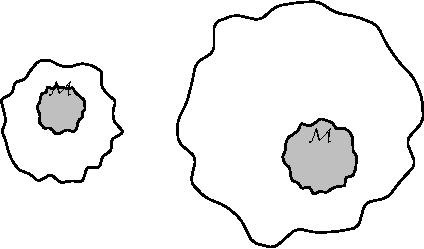
\includegraphics[width=\textwidth]{C:/Users/Jeffro/Documents/GitHub/Covariatesets/Diagrams/Identification.pdf}
  \caption{A model $\mathcal{M}$ is a set of structures that forms a proper subset of the class of all structures $\mathcal{S}$. Each structure in $\mathcal{M}$ generates a probability distribution in the class of all probability distributions (of observable variables) $\mathcal{P}$. Then the image $\mathcal{I}$ is the set of all probability distributions that are generated by structures in $\mathcal{M}$.}
  \label{fig:model}
  \end{subfigure}
\begin{subfigure}{0.8\textwidth}
  \centering
  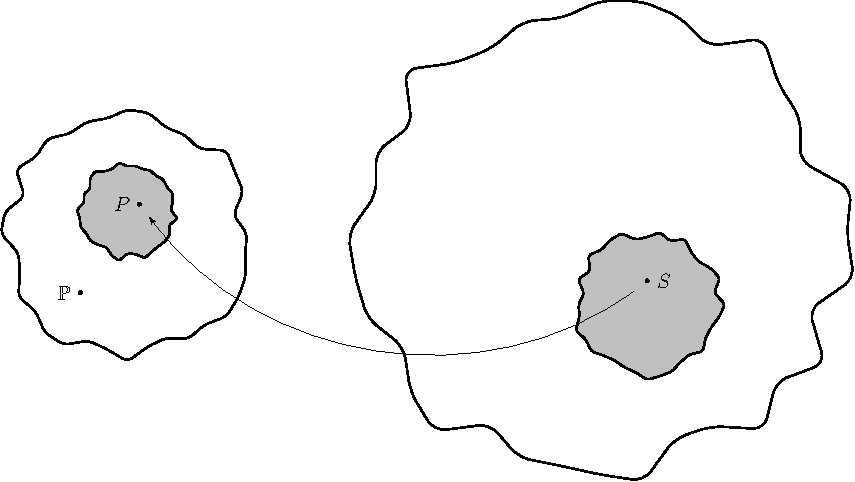
\includegraphics[width=\textwidth]{C:/Users/Jeffro/Documents/GitHub/Covariatesets/Diagrams/Observationalrestrictiveness.pdf}
  \caption{A structure $S$ is incompatible with data if it generates a probability distribution (of observable variables) $P$ that is distinct from a realised probability distribution $\mathbb{P}$. If all structures in $\mathcal{M}$ are incompatible with data then $\mathcal{M}$ is said to be observationally restrictive, and is falsified. This condition is equivalent to $\mathbb{P}\in\mathcal{P}\setminus\mathcal{I}$.}
  \label{fig:obs.restrict}
  \end{subfigure}
\caption{Structures, models, probability distributions (of observable variables), and falsifiability.}
\label{fig:models}
\end{figure}
%==================================================%
\begin{figure}[p]
\centering
\begin{subfigure}{0.8\textwidth}
  \centering
  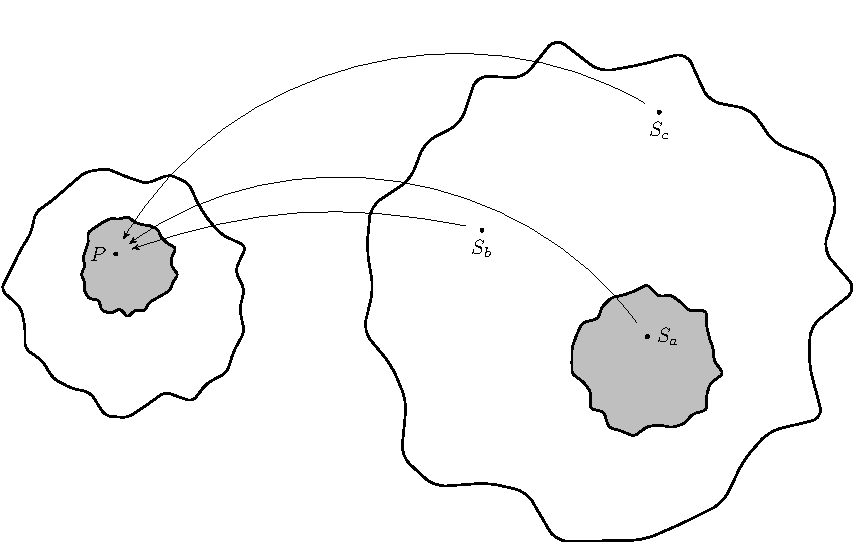
\includegraphics[width=\textwidth]{C:/Users/Jeffro/Documents/GitHub/Covariatesets/Diagrams/Pointidentification.pdf}
  \caption{A model $\mathcal{M}$ is said to identify a structure $S$ if the probability distribution (of observable variables) $P$ that is generated by $S$ is distinct from those generated by other structures in $\mathcal{M}$. The structures $S_a$, $S_b$ and $S_c$ are said to be observationally equivalent as they all generate $P$ but $S_b$ and $S_c$ are not admitted by $\mathcal{M}$. As $S_a$ is the only structure that is admitted by $\mathcal{M}$ and that generates $P$, $S_a$ is identified by $\mathcal{M}$. For completeness, $\mathcal{M}$ is said to be uniformly identifying if it identifies each structure that it admits.}
  \label{fig:identify}
  \end{subfigure}
  \begin{subfigure}{0.8\textwidth}
  \centering
  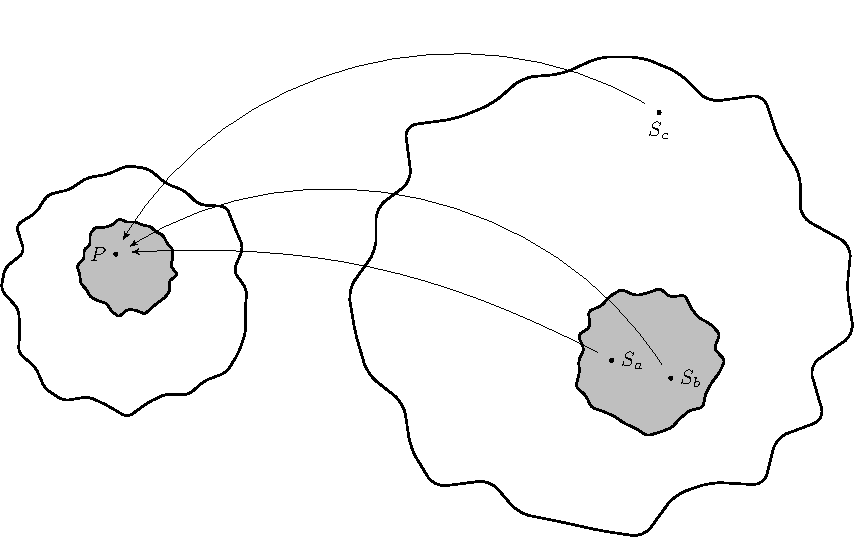
\includegraphics[width=\textwidth]{C:/Users/Jeffro/Documents/GitHub/Covariatesets/Diagrams/Setidentification.pdf}
  \caption{As $S_a$ and $S_b$ are observationally equivalent and are both admitted by $\mathcal{M}$ then $\mathcal{M}$ does not identify either $S_a$ or $S_b$. Nonetheless, as $\mathcal{M}$ restricts the set of observationally equivalent structures that generate $P$ to $S_a$ and $S_b$ then $\mathcal{M}$ partially identifies $S_a$ (and $S_b$ to within $\lbrace S_a,S_b\rbrace$).}
  \label{fig:partial}
  \end{subfigure}
\caption{Identification and non-identification of a structure, and partial identification of a structure.}
\label{fig:identification}
\end{figure}
%==================================================%
\begin{figure}[p]
\centering
\begin{subfigure}{0.8\textwidth}
  \centering
  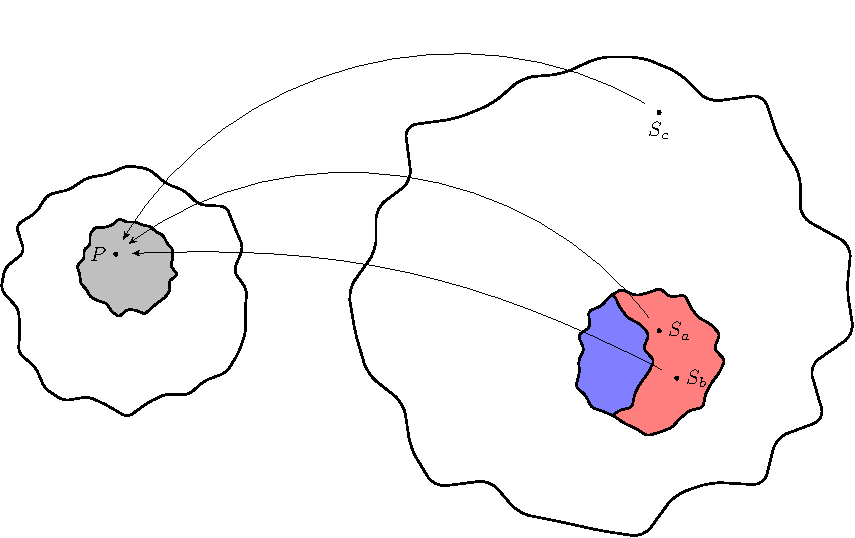
\includegraphics[width=\textwidth]{C:/Users/Jeffro/Documents/GitHub/Covariatesets/Diagrams/Characteristic.pdf}
  \caption{A structural characteristic $\chi$ is a function of a structure $S$. A model $\mathcal{M}$ can be partitioned such that structures in a partition deliver the same value for $\chi$. Structures in the red partition $\color{red}\mathcal{M}$ deliver the value $a$ for $\chi$, and structures in the red partition $\color{blue}\mathcal{M}$ deliver the value $b$ for $\chi$. If $\chi$ is constant across all observationally equivalent structures that $\mathcal{M}$ admits then $\mathcal{M}$ is said to identify $\chi$. As $\chi(S_a)$ is equal to $\chi(S_b)$ (is equal to $a$) $\mathcal{M}$ identifies $\chi$.}
  \label{fig:characteristic}
  \end{subfigure}
  \begin{subfigure}{0.8\textwidth}
  \centering
  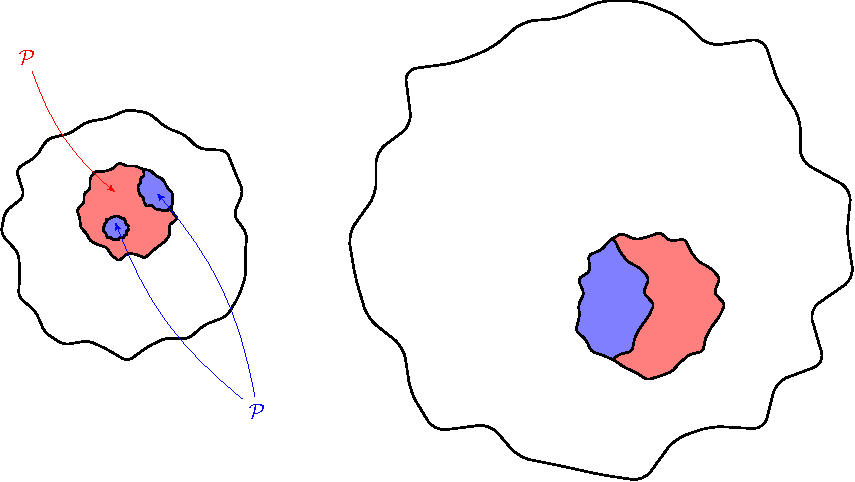
\includegraphics[width=\textwidth]{C:/Users/Jeffro/Documents/GitHub/Covariatesets/Diagrams/Uniform.pdf}
  \caption{If $\mathcal{M}$ identifies $\chi$ for all structures in $\mathcal{M}$ then $\mathcal{M}$ is said to uniformly identify $\chi$. The class of all probability distributions (of observable variables) is partitioned into the blue partition $\color{red}\mathcal{P}$ and into the red partition $\color{blue}\mathcal{P}$. Probability distributions in $\color{red}\mathcal{P}$ are generated by (potentially many) structures in $\color{red}\mathcal{M}$, and probability distributions in $\color{blue}\mathcal{P}$ are generated by (potentially many) structures in $\color{blue}\mathcal{M}$. It is important that the number of partitions in $\mathcal{M}$ and in $\mathcal{P}$ are equal, although that number can be countably infinite. In the context of Figure~\ref{fig:uniform} $\mathcal{M}$ uniformly identifies $\chi$ since observationally equivalent structures that $\mathcal{M}$ admits are in the same colour of $\mathcal{M}$. More conveniently, whether $\mathcal{M}$ uniformly identifies $\chi$ can be determined by the existence of an identifying correspondence $G$, a functional. $\color{red}P$ is a probability distribution in $\color{red}\mathcal{P}$, and $\color{blue}P$ is a probability distribution in $\color{blue}\mathcal{P}$. Then $\mathcal{M}$ uniformly identifies $\chi$ if the value of $G(\color{red}P\color{black})$ is $a$ and if the value of $G(\color{blue}P\color{black})$ is $b$, holding for any such $\color{red}P$ and $\color{blue}P$. Notice that if $\mathcal{M}$ uniformly identifies all $\chi$ then $\mathcal{M}$ also uniformly identifies structures.}
  \label{fig:uniform}
  \end{subfigure}
  \caption{The identification of structural characteristics, and identifying correspondences.}
  \label{fig:characteristics}
\end{figure}
%==================================================%
\begin{figure}[p]
\centering
\begin{subfigure}{0.8\textwidth}
\centering
\caption{A structural characteristic $\chi$ is a function of a structure $S$. A model $\mathcal{M}$ can be partitioned such that structures in a partition deliver the same value for $\chi$. Structures in the red partition $\color{red}\mathcal{M}$ deliver the value $a$ for $\chi$, structures in the blue partition $\color{blue}\mathcal{M}$ deliver the value $b$ for $\chi$, and structures in the yellow partition $\color{yellow}\mathcal{M}$ deliver the value $c$ for $\chi$. The class of all probability distributions (of observable variables) $\mathcal{P}$ is partitioned into the red partition $\color{red}\mathcal{P}$, into the blue partition $\color{blue}\mathcal{P}$, into the yellow partition $\color{yellow}\mathcal{P}$ and into the grey partition $\color{gray}\mathcal{P}$. Probability distributions in a colour of $\mathcal{P}$ are generated by (potentially many) structures in the same colour of $\mathcal{M}$; the exception is probability distributions in $\color{gray}\mathcal{P}$ which are generated by (potentially many) structures in $\color{red}\mathcal{M}$ and in $\color{yellow}\mathcal{M}$. $P$ is a probability distribution in $\mathcal{P}$ with probability distributions defined similarly for each colour in $\mathcal{P}$.}
\end{subfigure}
\begin{subfigure}{0.8\textwidth}
  \centering
  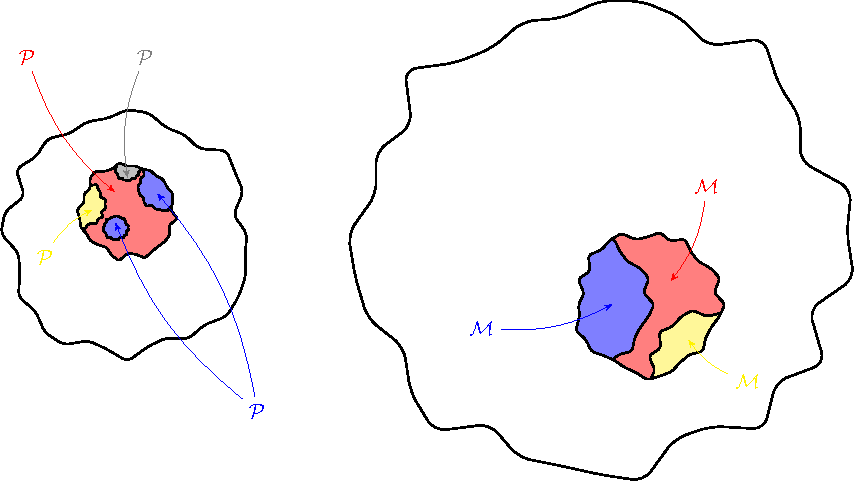
\includegraphics[width=\textwidth]{C:/Users/Jeffro/Documents/GitHub/Covariatesets/Diagrams/Partial.pdf}
  \caption{That probability distributions in $\color{gray}\mathcal{P}$ are generated by structures in $\color{red}\mathcal{M}$ and in $\color{yellow}\mathcal{M}$ creates a complication; the value of $\chi$ is not constant across observationally equivalent structures that $\mathcal{M}$ admits and that generate a probability distribution in $\color{gray}\mathcal{P}$. So $\mathcal{M}$ does not uniformly identify $\chi$. Consideration of the identifying correspondence $G$ determines that this corresponds to there being structures in $\mathcal{M}$ for which $G$ does not deliver the value of $\chi$ when applied to the probability distributions that these structures generate. Nonetheless, if $\mathcal{M}$ restricts the set of values of $\chi$ for any probability distribution in $\mathcal{P}$ then $\mathcal{M}$ does have some non-trivial identifying power for $\chi$. Then $\mathcal{M}$ is said to uniformly partially identify $\chi$ if $\mathcal{M}$ and $\mathcal{P}$ can each be partitioned into countably many disjoint subsets and that a probability distribution in a partition of $\mathcal{P}$ is not generated by a structure in at least one partition of $\mathcal{M}$, holding for any such partition of $\mathcal{P}$. In the context of Figure~\ref{fig:partials} $\color{red}\mathcal{M}$ identifies $\chi$ up to $\lbrace a,c\rbrace$, $\color{blue}\mathcal{M}$ identifies $\chi$ uniquely to $b$, and $\color{yellow}\mathcal{M}$ identifies $\chi$ up to $\lbrace a,c\rbrace$. Each partition of $\mathcal{P}$ includes probability distributions that are generated by structures in at least one partition of $\mathcal{M}$. Equivalently, if $G$ is permitted to be a multivalued functional (or one-to-many) then $\mathcal{M}$ uniformly partially identifies $\chi$ if $G$ exists and if $G(P)$ contains the set of values of $\chi$ that are delivered by structures that generate $P$, holding for all such $P$. A caveat must be applied here; $G$ cannot be trivial in the sense that it is constant across all such $P$. Clearly this definition of $G$ does not exclude the possibility that there is multiplicity of identifying correspondences that satisfy this property. Sharpness is a desirable property in such circumstances; a functional $G$ that can be shown to deliver smaller sets according to some well-defined distance measure across all possible $P$ (and that satisfies the properties above) should be preferred to any alternative identifying correspondence.}
  \label{fig:partial1}
  \end{subfigure}
  \caption{Partial identification of a structural characteristic.}
  \label{fig:partials}
\end{figure}
%==================================================%
\begin{figure}[p]
\centering
\begin{subfigure}{0.4\textwidth}
  \centering
  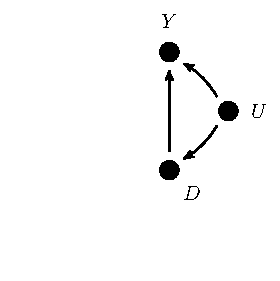
\includegraphics[width=\textwidth]{C:/Users/Jeffro/Documents/GitHub/Covariatesets/Diagrams/Indistinguishable1.pdf}
  \label{fig:indistinguishable1}
  \end{subfigure}
  \begin{subfigure}{0.4\textwidth}
  \centering
  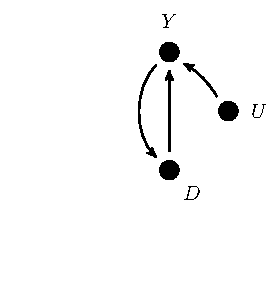
\includegraphics[width=\textwidth]{C:/Users/Jeffro/Documents/GitHub/Covariatesets/Diagrams/Indistinguishable2.pdf}
  \label{fig:indistinguishable2}
  \end{subfigure}
\begin{subfigure}{0.8\textwidth}
  \caption{The left- and right-hand panels show directed acyclic graphs that are able to represent the same probability distribution of $(Y,D)$. In the left-hand panel, $U$ causes $Y$ and $D$. The left-hand panel is a representation of selection in that particular values of $D$ are strongly associated with particular values of $Y$ independently of the causal effect of $D$. In the right-hand panel, $U$ causes $Y$ but has an indirect effect on $D$ through $Y$. The right-hand panel is a representation of simultaneity in that $Y$ is both a cause of and an effect of $D$. The equivalence between the two directed acyclic graphs is that $Y$ can always be written as $\xi(D,U)$ for $\xi : \mathcal{R}_D\times\mathcal{R}_U\rightarrow\mathcal{R}_Y$ (provided that the right-hand panel is convergent).}
  \end{subfigure}
   \begin{subfigure}{0.4\textwidth}
  \centering
  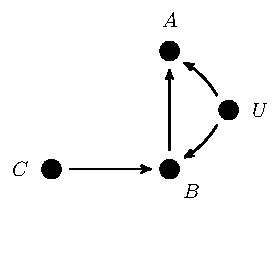
\includegraphics[width=\textwidth]{C:/Users/Jeffro/Documents/GitHub/Covariatesets/Diagrams/Exogenous1.pdf}
  \label{fig:exogenous1}
  \end{subfigure}
   \begin{subfigure}{0.4\textwidth}
  \centering
  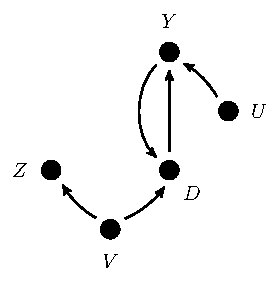
\includegraphics[width=\textwidth]{C:/Users/Jeffro/Documents/GitHub/Covariatesets/Diagrams/Exogenous2.pdf}
  \label{fig:exogenous2}
  \end{subfigure}
  \begin{subfigure}{0.8\textwidth}
  \caption{To recover the causal effect of $D$ on $Y$, it is necessary that there exists an external and measurable factor that causes variation in $D$. This external and measurable factor is known as an instrumental variable. In the left-hand panel, $Z$ causes $D$. It is convenient to think of $Z$ as a switch that forces $D$ to take particular values. The difference between the value of $Y$ when $Z$ is $\mathtt{on}$ versus when $Z$ is $\mathtt{off}$ is the causal effect of $D$ on $Y$. In the right-hand panel, it is $V$ that causes $D$ ($V$ is unobservable). As $V$ causes $D$ and $Z$, it may be sufficient to look at $Z$ to measure exogenous variation in $D$ (although it is not always). As such, the causal effect of $D$ on $Y$ is recoverable using variation in $Z$. This is an important point about the nature of an instrumental variable; namely, that the relationship between $D$ and $Z$ need not be causal.}
  \end{subfigure}
  \caption{A note on causality.}
  \label{fig:causality}
\end{figure}
%==================================================%
\begin{figure}[p]
\centering
\begin{subfigure}{0.8\textwidth}
\caption{Suppose that $\color{blue}\theta_n^u(z)\color{black}$ and $\color{red}\theta_n^u(z')\color{black}$ are estimates of upper bounds on $\mathbb{E}[Y(0)]$. Similarly, suppose that $\color{blue}\phi_n^u(z)\color{black}$ and $\color{red}\phi_n^u(z')\color{black}$ are one-sided $1-\alpha$ confidence regions for $\color{blue}\theta_n^u(z)\color{black}$ and $\color{red}\theta_n^u(z')\color{black}$. $\color{red}\phi_n^u(z')\color{black}>\color{blue}\phi_n^u(z')\color{black}$ if there is greater variation in the estimate of $\color{blue}\theta_n^u(z)\color{black}$ (if there are fewer observations of $z$ than $z'$, say).}
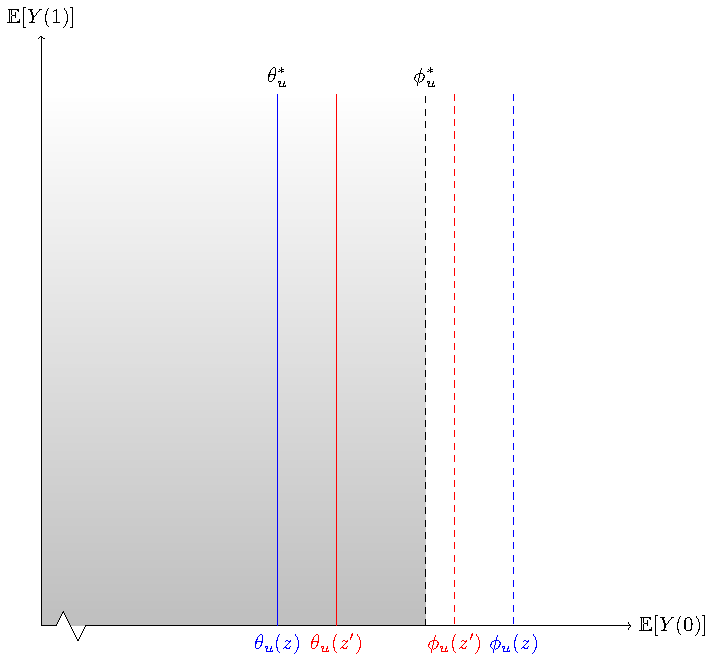
\includegraphics[width=\textwidth]{C:/Users/Jeffro/Documents/GitHub/Covariatesets/Diagrams/Confidence.pdf}
\caption{As $\color{blue}\theta_n^u(z)\color{black}$ and $\color{red}\theta_n^u(z')\color{black}$ are both binding constraints on $\mathbb{E}[Y(0)]$, the minimum of these upper bounds must be binding. The minimum upper bound is written as $\theta^u_n$ and is $\color{blue}\theta_n^u(z)\color{black}$. The inferential problem is to determine $\phi_n^u$, which satisfies 
$\mathbb{P}(\theta_n>\phi_n^u)=\alpha$. A na{\"i}ve approach would be to look only at the one-sided $1-\alpha$ confidence region for $\color{blue}\theta_n^u(z)\color{black}$, which is $\color{blue}\phi_n^u(z)\color{black}$. This approach ignores variation in $\color{red}\theta_n^u(z')\color{black}$. An equally na{\"i}ve approach would be to simply add aggregate variation to $\color{blue}\theta_n^u(z)\color{black}$. In other words, to add the weighted average of $\color{blue}\phi_n^u(z)\color{black}-\color{blue}\theta_n^u(z)\color{black}$ and $\color{red}\phi_n^u(z')\color{black}-\color{red}\theta_n^u(z')\color{black}$ to $\color{blue}\theta_n^u(z)\color{black}$. This approach is standard but fails in this case because it does not account for the fact that $\color{blue}\theta_n^u(z)\color{black}<\color{red}\theta_n^u(z')\color{black}$. Inference must account for the fact that upward variation in $\color{red}\theta_n^u(z')\color{black}$ does not matter so long as $\color{blue}\theta_n^u(z)\color{black}<\color{red}\theta_n^u(z')\color{black}$; equivalently, that $\color{red}\theta_n^u(z')\color{black}$ is a one-sided $1-\gamma$ confidence region for $\color{blue}\theta_n^u(z)\color{black}$ for $\gamma>\alpha$. \cite{cHlr13} solves the inferential problem by adjusting the critical value that is associated with the one-sided $1-\alpha$-confidence region. That is, \cite{cHlr13} adjusts $k$ such that $k$ that solves $\mathbb{P}(\theta_n>\color{blue}\theta_n^u(z)\color{black}+k\sigma)=\alpha$. The solution for $k$ yields $\phi_n^u$ with the one-sided $1-\alpha$ confidence region for $\theta_n^u$ given by the grey area. The distribution of $\theta_n^u$ over repeated samples is non-standard in this case and the bootstrap is  not necessarily consistent \citep{bU10}.} 
\end{subfigure}
\caption{A note on the inferential problem.}
\label{fig:confidence}
\end{figure}
\begin{figure}[p]
\centering
\begin{subfigure}{0.8\textwidth}
\caption{Suppose that the admissible set of values of $(\mathbb{E}[Y(0)],\mathbb{E}[Y(1)])$ is given by the blue rectangle, and that the $1-\alpha$-confidence region for this set is the union of the blue rectangle and the red polygon. }
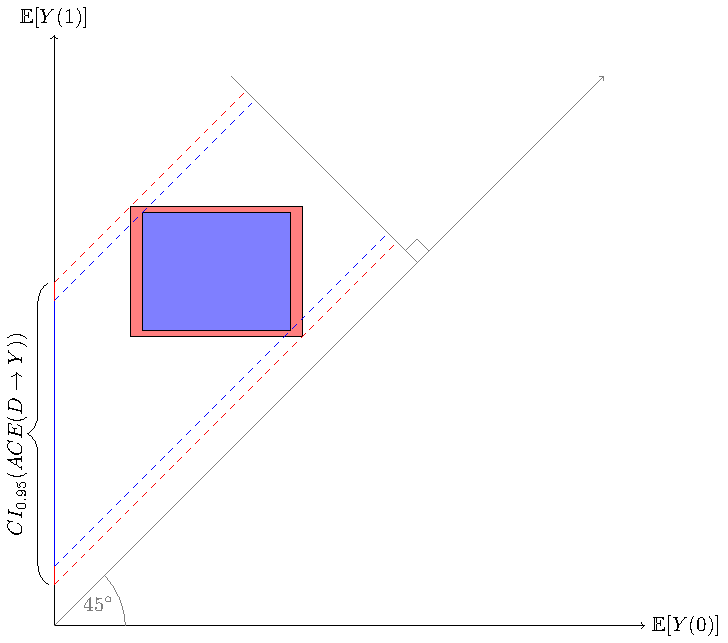
\includegraphics[width=\textwidth]{C:/Users/Jeffro/Documents/GitHub/Covariatesets/Diagrams/ACE.pdf}
\caption{It is possible to recover $ACE(D\rightarrow Y)$ from the plot. First, note that $ACE(D\rightarrow Y)$ is increasing in the $y$-direction and is decreasing in the $x$-direction. Second, note that $ACE(D\rightarrow Y)$ is constant along any line with unit gradient. Third, note that the value of $ACE(D\rightarrow Y)$ along any line with unit gradient is dependent upon the value of the intercept of this line. Fourthly, note that a projection from the normal of a line with unit gradient is a line that has unit gradient. For example, the blue dashed line is a projection from the normal of the $45^\circ$ line; notice that the blue dashed line is parallel to the $45^\circ$ line. Fifth, note that any projection from the normal of the $45^\circ$ line that passes through the blue rectangle is an admissible value of $(\mathbb{E}[Y(0)],\mathbb{E}[Y(1)])$; equivalently, that any projection from the normal of the $45^\circ$ line that passes through the union of the blue rectangle and the red polygon is in the $1-\alpha$ confidence region of $(\mathbb{E}[Y(0)],\mathbb{E}[Y(1)])$. Together these five facts suggest that the admissible set of values of $ACE(D\rightarrow Y)$ and its $1-\alpha$ confidence region can be recovered from the projection from the normal of the $45^\circ$ line onto the $y$-axis. This method gives a geometric interpretation to $ACE(D\rightarrow Y)$.}
\end{subfigure}
\caption{A note on recovering the average causal effect.}
\label{fig:ace}
\end{figure}
%==================================================%
%% Diagrams
\invisiblesection{Tables}
%==================================================%
\begin{sidewaystable}[p]
\centering
\begin{tabular}{lcrcrcrcr}
\toprule
&	& \multicolumn{7}{c}{Bound} \\
\cmidrule(r){2-9}	
	$\mathcal{R}_Z$	&	&	$\theta_{n}^{0-}$	&	&	$\theta_n^{1-}$	&	&	$\theta_{n}^{0+}$	&	&	$\theta_n^{1+}$\\
\midrule
\phantom{$\text{Male-Female}\cup\text{Female-Male}\cup\text{Female-Female}$}\\
%1	
$\text{Male-Male}\cup\text{Female-Female}$	&	&	$[0.533,0.721]$	&	&	$[0.189,0.524]$	&	&	$[0.374,0.524]$	&	&	$[0.533,0.775]$
\\
$\text{Male-Female}\cup\text{Female-Male}$	&	&	\color{blue}$[0.530,0.723]$	&	&	\color{blue}$[0.187,0.527]$	&	&	\color{blue}$[0.371,0.527]$	&	&	\color{blue}$[0.530,0.777]$\\
\\
%2
$\text{Male-Male}$	&	&	$[0.530,0.731]$	&	&	$[0.182,0.523]$	&	&	$[0.359,0.523]$	&	&	$[0.530,0.778]$
\\
$\text{Male-Female}\cup\text{Female-Male}\cup\text{Female-Female}$	&	&	\color{blue}$[0.528,0.733]$	&	&	\color{blue}$[0.179,0.527]$	&	&	\color{blue}$[0.357,0.527]$	&	&	\color{blue}$[0.528,0.781]$\\
\\
%3
$\text{Female-Female}$	&	&	$[0.529,0.729]$	&	&	$[0.196,0.524]$	&	&	$[0.362,0.524]$	&	&	$[0.529,0.771]$
\\
$\text{Male-Male}\cup\text{Male-Female}\cup\text{Female-Male}$	& &\color{blue}$[0.527,0.731]$	&	&	\color{blue}$[0.193,0.529]$	&	&	\color{blue}$[0.360,0.529]$	&	&	\color{blue}$[0.527,0.774]$\\	
\\
%4
$\text{Male-Male}$&	&	$[0.533,0.721]$	&	&	$[0.196,0.523]$	&	&	$[0.374,0.523]$	&	&	$[0.533,0.771]$
\\
$\text{Female-Female}$ & &\color{blue}$[0.530,0.723]$	&	&	\color{blue}$[0.192,0.528]$	&	&	\color{blue}$[0.371,0.528]$	&	&	\color{blue}$[0.530,0.775]$\\
$\text{Male-Female}\cup\text{Female-Male}$\\	
\\
%5
$\text{Male-Male}$&	&	$[0.536,0.718]$	&	&	$[0.196,0.523]$	&	&	$[0.376,0.523]$	&	&	$[0.536,0.771]$
\\
$\text{Female-Female}$& &\color{blue}$[0.531,0.722]$	&	&	\color{blue}$[0.193,0.528]$	&	&	\color{blue}$[0.372,0.528]$	&	&	\color{blue}$[0.531,0.775]$\\
$\text{Male-Female}$ \\
$\text{Female-Male}$\\	
	\\
\bottomrule
\end{tabular}
\caption{$95\%$ confidence regions for parameters $(1-p)$ constructed using $97.5\%$ one-sided confidence. }
\label{tbl:setssame}
\end{sidewaystable}
%==================================================%
\begin{sidewaystable}[p]
\centering
\begin{tabular}{lcrcr}
\toprule
&	& \multicolumn{3}{c}{Bound} \\
\cmidrule(r){2-5}	
	$\mathcal{R}_Z$	&	&	$\theta_{n}^{0-}$	&	&	$\theta_n^{1-}$	\\
\midrule
\phantom{$\text{Male-Female}\cup\text{Female-Male}\cup\text{Female-Female}$}\\
%6
$\text{Multiple birth}$&	&	$[0.529,0.733]$	&	&	$0.476$\\
$\text{Single birth}$& &\color{blue}$[0.526,0.734]$	&	&	\color{blue}$[0.460,0.498]$\\
\\
%7
$\text{Multiple birth}$&	&	$[0.534,0.718]$	&	&	$0.476$\\
$\text{Single birth}\cap(\text{Male-Male}\cup\text{Female-Female})$& &\color{blue}$[0.530,0.721]$	&	&	\color{blue}$[0.460,0.498]$\\
$\text{Single birth}\cap(\text{Male-Female}\cup\text{Female-Male})$\\
\\
%8
$\text{Multiple birth}$&	&	$[0.537,0.716]$	&	&	$0.476$\\
$\text{Single birth}\cap\text{Male-Male}$& &\color{blue}$[0.532,0.720]$	&	&	\color{blue}$[0.460,0.498]$\\
$\text{Single birth}\cap\text{Female-Female}$\\
$\text{Single birth}\cap\text{Male-Female}$ \\
$\text{Single birth}\cap\text{Female-Male}$\\
	\\
\bottomrule
\end{tabular}
\caption{}
\label{tbl:setsmult}
\end{sidewaystable}
%==================================================%
\begin{table}[p]
\centering
\begin{tabular}{lcrcr}
\toprule
&	& \multicolumn{3}{c}{Bound} \\
\cmidrule(r){2-5}	
	$\mathcal{R}_Z$	&	&	$ACE_n(D\rightarrow Y)^-$	&	&	$ACE_n(D\rightarrow Y)^+$\\
\midrule
\phantom{$\text{Male-Female}\cup\text{Female-Male}\cup\text{Female-Female}$}\\
%1	
$\text{Male-Male}\cup\text{Female-Female}$	&	&	$[-0.532,-0.009]$	&	&	$[0.009,0.401]$	\\
$\text{Male-Female}\cup\text{Female-Male}$	&	&	\color{blue}$[-0.537,-0.002]$	&	&	\color{blue}$[0.002,0.406]$	\\
\\
%2
$\text{Male-Male}$	&	&	$[-0.549,-0.007]$	&	&	$[0.007,0.419]$	\\
$\text{Male-Female}\cup\text{Female-Male}\cup\text{Female-Female}$	&	&	\color{blue}$[-0.555,0.001]$	&	&	\color{blue}$[-0.001,0.425]$\\
\\
%3
$\text{Female-Female}$	&	&	$[-0.533,-0.005]$	&	&	$[0.005,0.409]$	\\
$\text{Male-Male}\cup\text{Male-Female}\cup\text{Female-Male}$	& &\color{blue}$[-0.539,0.003]$	&	&	\color{blue}$[-0.003,0.415]$\\	
\\
%4
$\text{Male-Male}$&	&	$[-0.525,-0.010]$	&	&	$[0.010,0.397]$	\\
$\text{Female-Female}$ & &\color{blue}$[-0.531,-0.001]$	&	&	\color{blue}$[0.002,0.404]$\\
$\text{Male-Female}\cup\text{Female-Male}$\\	
\\
%5
$\text{Male-Male}$&	&	$[-0.523,-0.013]$	&	&	$[0.013,0.395]$	\\
$\text{Female-Female}$& &\color{blue}$[-0.530,-0.003]$	&	&	\color{blue}$[0.003,0.403]$	\\
$\text{Male-Female}$ \\
$\text{Female-Male}$\\	
	\\
\bottomrule
\end{tabular}
\caption{$95\%$ confidence regions for parameters $ACE$ constructed using $98.75\%$ one-sided confidence for each parameter.}
\label{tbl:acesame}
\end{table}
%==================================================%
\begin{table}[p]
\centering
\begin{tabular}{lcr}
\toprule
&	& \multicolumn{1}{c}{Bound} \\
\cmidrule(r){3-3}	
	$\mathcal{R}_Z$	&	&	$\theta_{n}^{0-}$\\
\midrule
\phantom{$\text{Male-Female}\cup\text{Female-Male}\cup\text{Female-Female}$}\\
%6
$\text{Multiple birth}$&	&	$[-0.256,-0.052]$\\
$\text{Single birth}$& &\color{blue}$[-0.277,-0.025]$	\\
\\
%7
$\text{Multiple birth}$&	&	$[-0.242,-0.057]$	\\
$\text{Single birth}\cap(\text{Male-Male}\cup\text{Female-Female})$& &\color{blue}$[-0.263,-0.029]$\\
$\text{Single birth}\cap(\text{Male-Female}\cup\text{Female-Male})$\\
\\
%8
$\text{Multiple birth}$&	&	$[-0.240,-0.061]$	\\
$\text{Single birth}\cap\text{Male-Male}$& &\color{blue}$[-0.262,-0.031]$	\\
$\text{Single birth}\cap\text{Female-Female}$\\
$\text{Single birth}\cap\text{Male-Female}$ \\
$\text{Single birth}\cap\text{Female-Male}$\\
	\\
\bottomrule
\end{tabular}
\caption{}
\label{tbl:acemult}
\end{table}
%==================================================%
%% Bibliography.
\newpage
\bibliographystyle{chicago}
\bibliography{\details Bibliography}
\end{document}